\section{FANUC setup}
The FANUC robot system required some setup and programming before it could be used as an FDM 3D printing platform. Most of the procedures and settings described in this section can be learned fairly quickly from the lab-style tutorials in \cite{app-programming}. Full documentation is available in the controller manual \cite{lr-handling-tool}.

All of the setup and programming associated with the FANUC controller is performed through the controller's attached "iPendant" teach pendant, pictured in Figure~\ref{fig:teach-pendant}. Note that using the teach pendant to move the robot in any way requires that the teach pendant's dead man's switch, shown in Figure~\ref{fig:deadman}, be depressed properly. The switch has three positions: un-depressed, partially depressed, and fully depressed. The switch is considered "released" and throws an error if it is un-depressed or fully depressed.

\begin{figure}
    \centering
    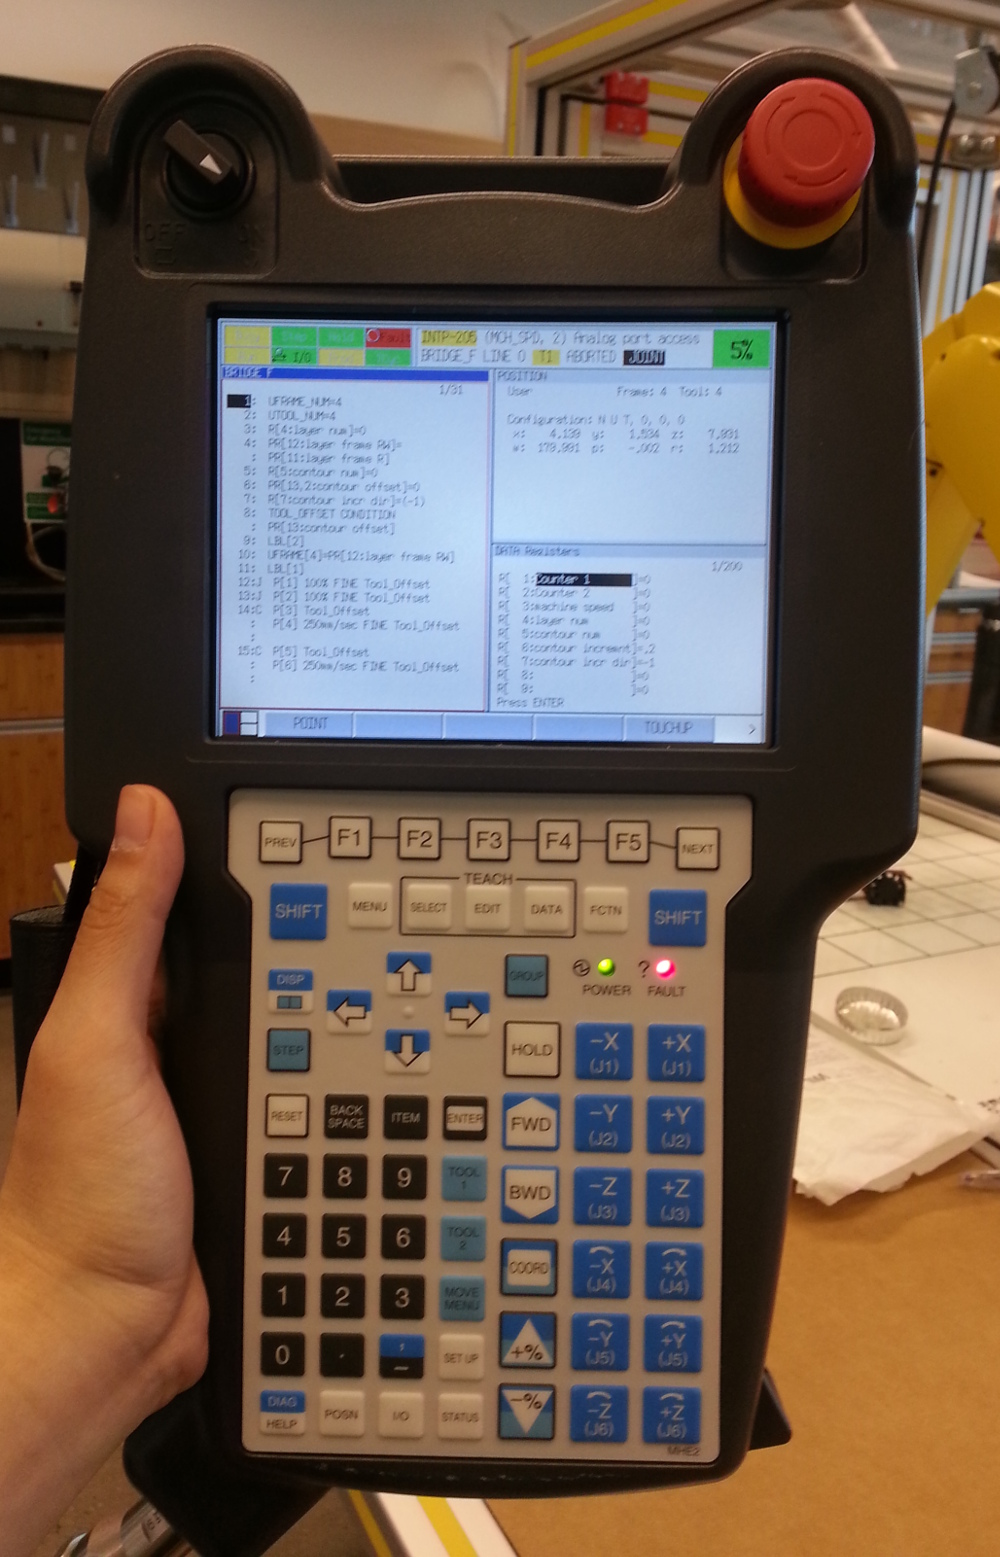
\includegraphics[width=.5\linewidth]{figures/teach-pendant}
    \caption{FANUC R30iA Mate Teach Pendant}
    \label{fig:teach-pendant}
\end{figure}

\begin{figure}
    \centering
    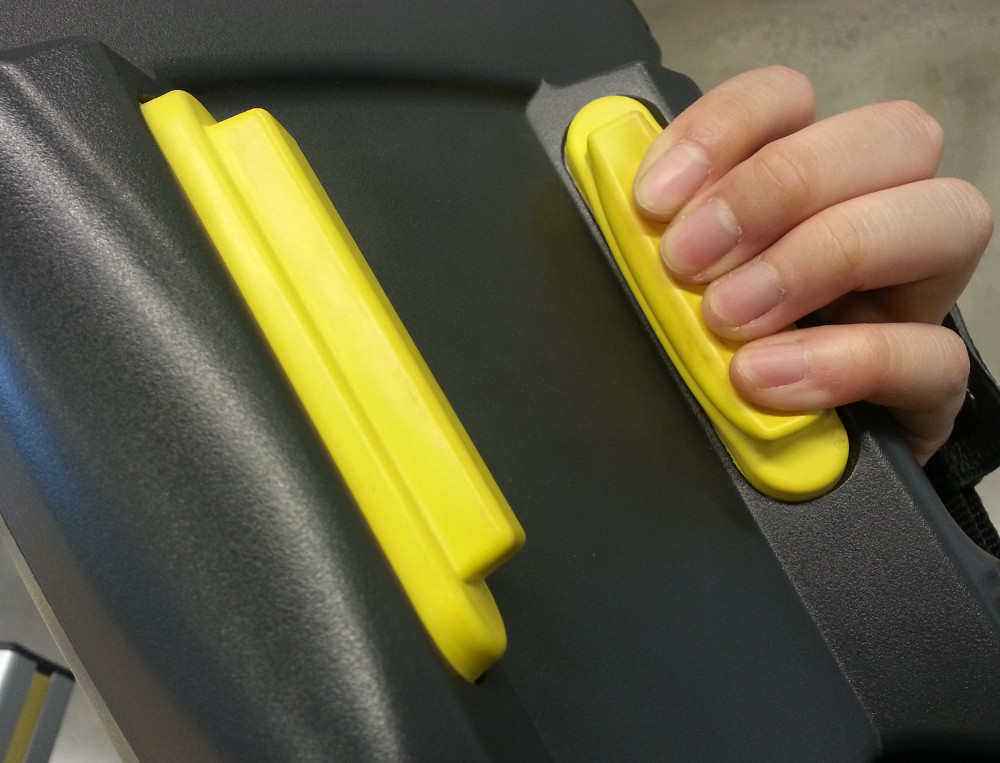
\includegraphics[width=.8\linewidth]{figures/deadman.jpg}
    \caption{Teach pendant dead man's switch, depressed properly.}
    \label{fig:deadman}
\end{figure}

\subsection{Frames}
The FANUC robot system makes several types of coordinate systems available for defining the robot position and attitude (orientation) in space. These include some pre-defined coordinate systems  that cannot be redefined \cite[sec 3.9]{lr-handling-tool}. The user may define custom coordinate systems attached to the robot or the workspace. These coordinate systems are called "frames" in the teach pendant interface.

It is entirely possible to create useful robot arm applications using only the pre-defined frames. However, doing so is usually computationally impractical. For the 3D printing application, a new tool coordinate system and user coordinate system were defined to simplify further programming.

\subsubsection{Tool frame}
The new tool frame is attached to the custom end effector with its origin at the tip of the extruder nozzle, at what is considered the TCP (tool center point). Defining a tool frame allows the user program robot motions by defining positions and orientations of the TCP only, which are likely the values of interest; the controller performs the inverse kinematic calculations to determine the required robot joint angles for each move. For this application, the tool frame will be especially important for maintaining the desired tool attitude relative to the surface of a curved-layer 3D-printed part in progress. 

The tool frame was defined using the Three Point Method described in \cite[sec~3.9.1]{lr-handling-tool}. The three reference positions (points) used are pictured in Figures~\ref{fig:tool-pt-1} through \ref{fig:tool-pt-3}. An elevated piece of scrap material was used as the tool center reference point to facilitate visual alignment with the nozzle and avoid over-extending the vision camera wire while jogging the robot to the desired approach angles.

\begin{figure}
    \centering
    \begin{subfigure}{.5\textwidth}
        \centering
            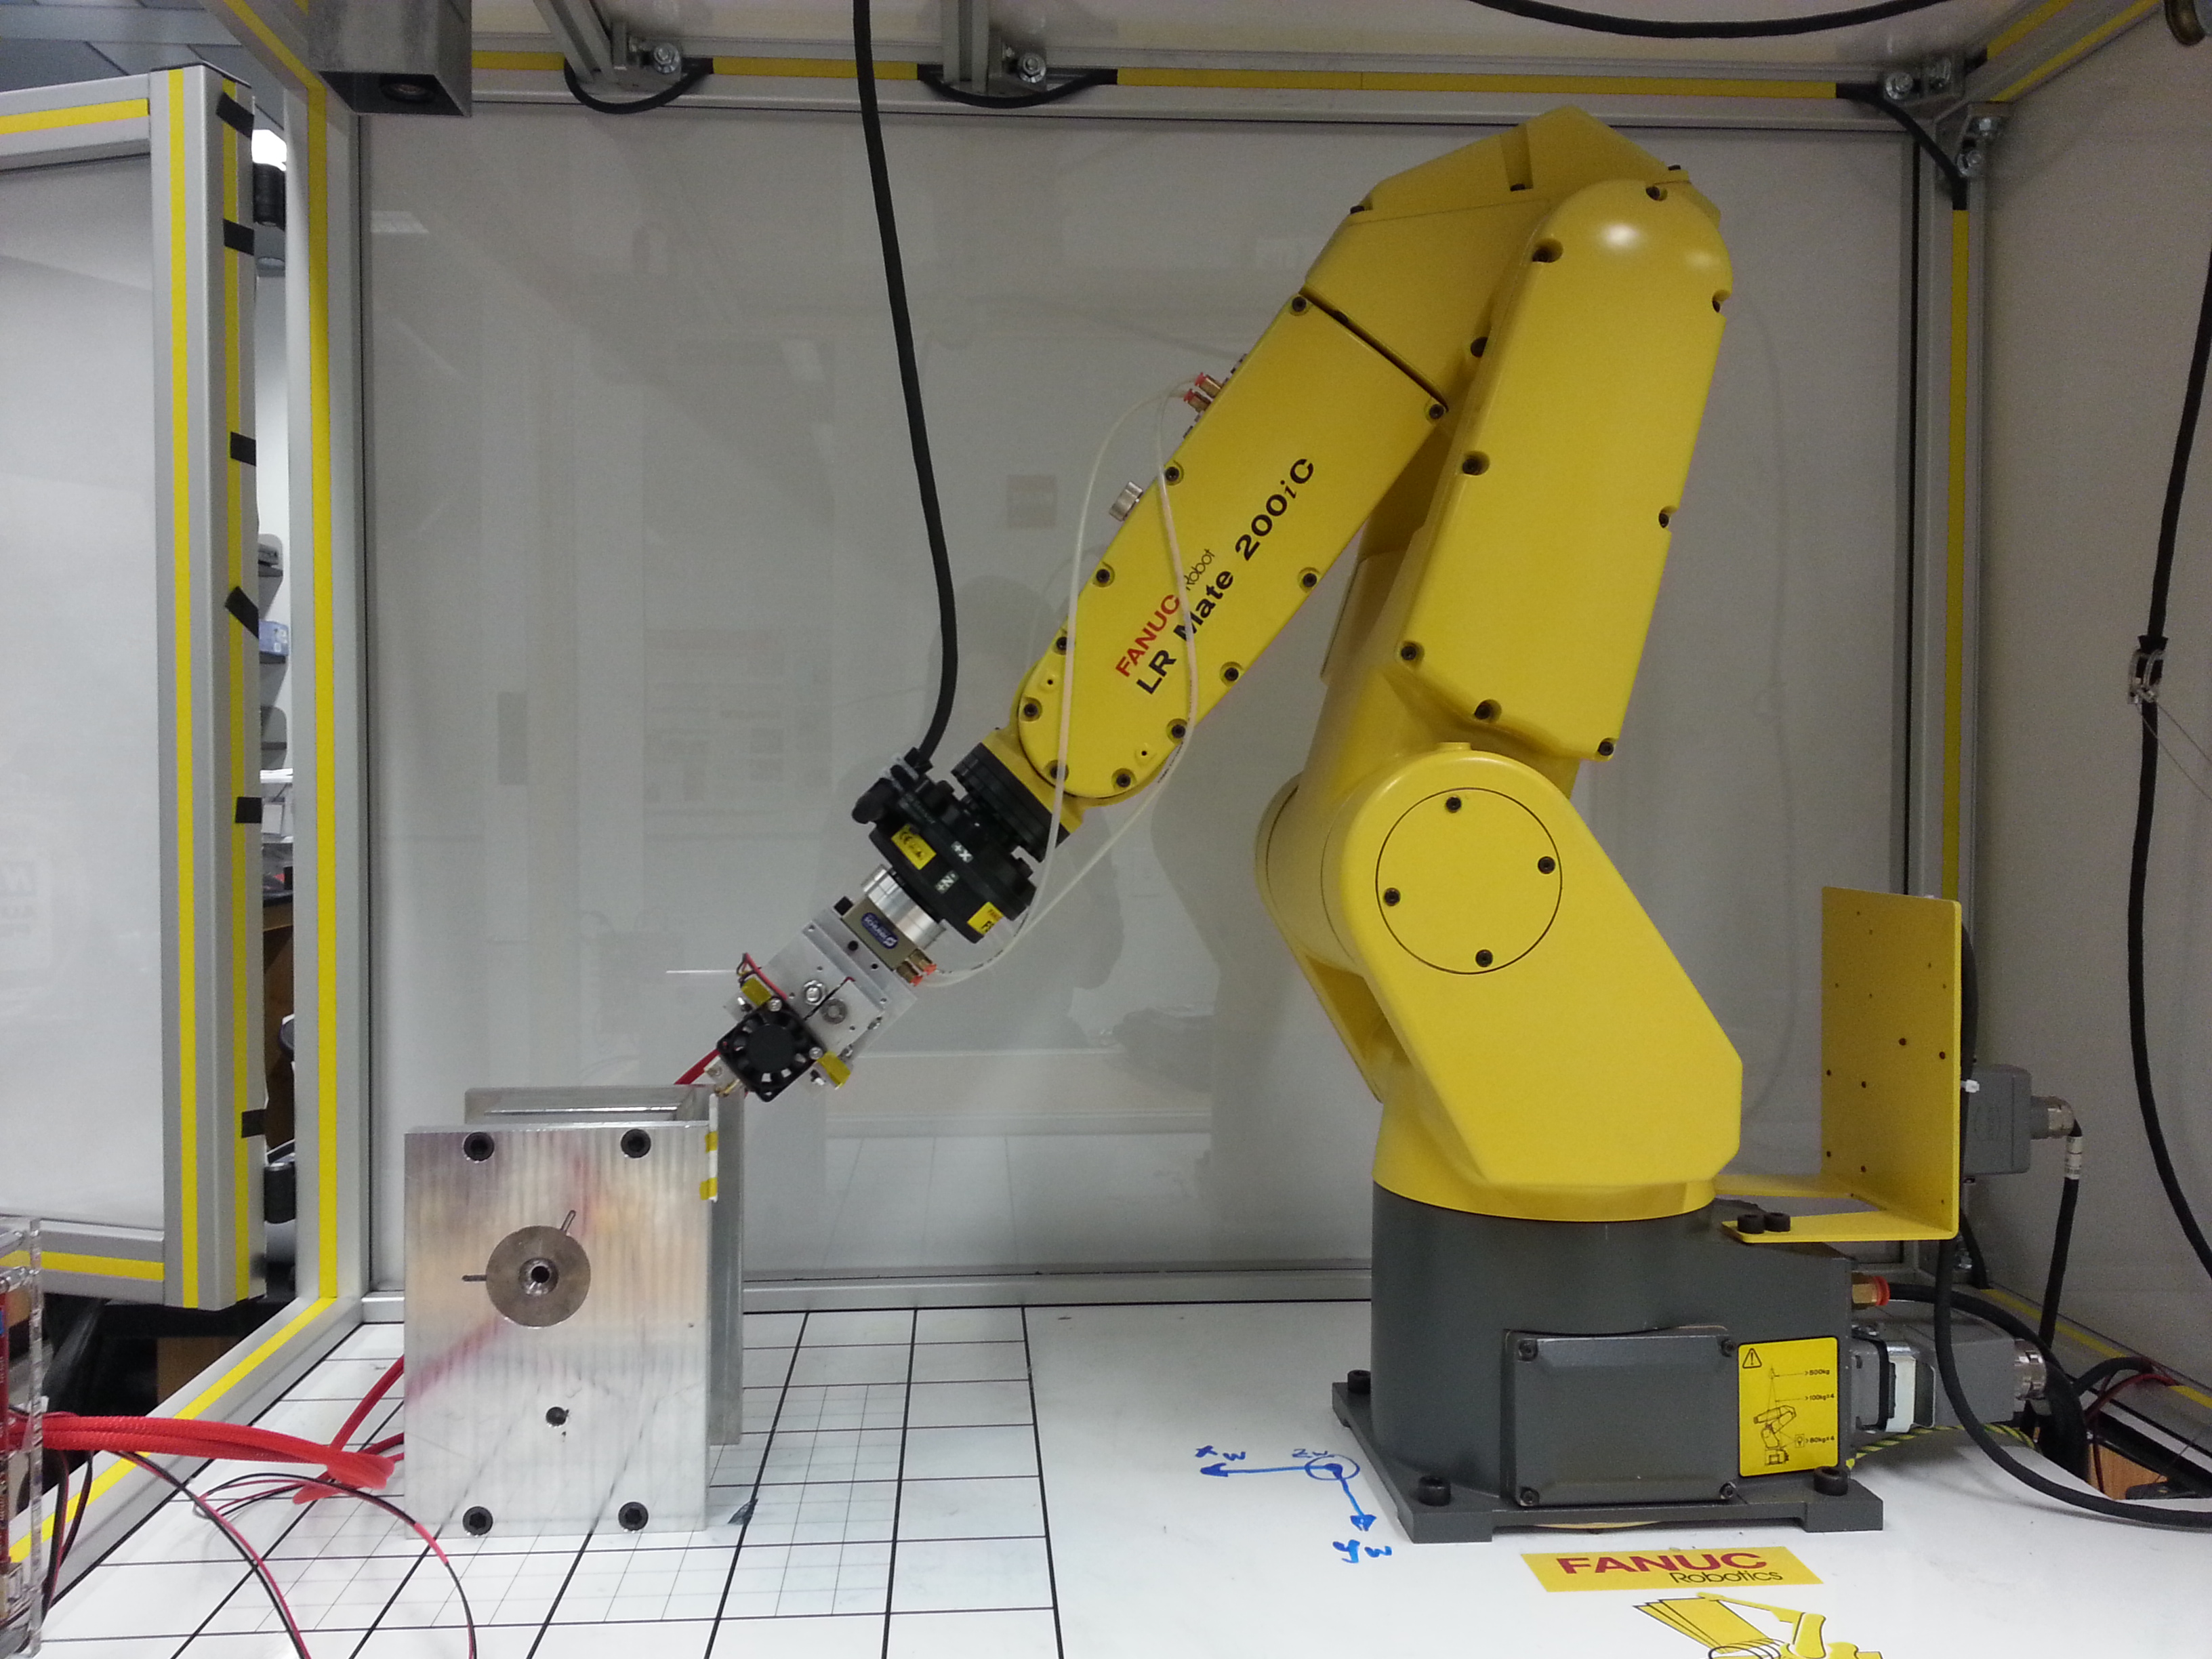
\includegraphics[width=.8\linewidth]{figures/tool-pt-1}
    \end{subfigure}%
    \begin{subfigure}{.5\textwidth}
        \centering
        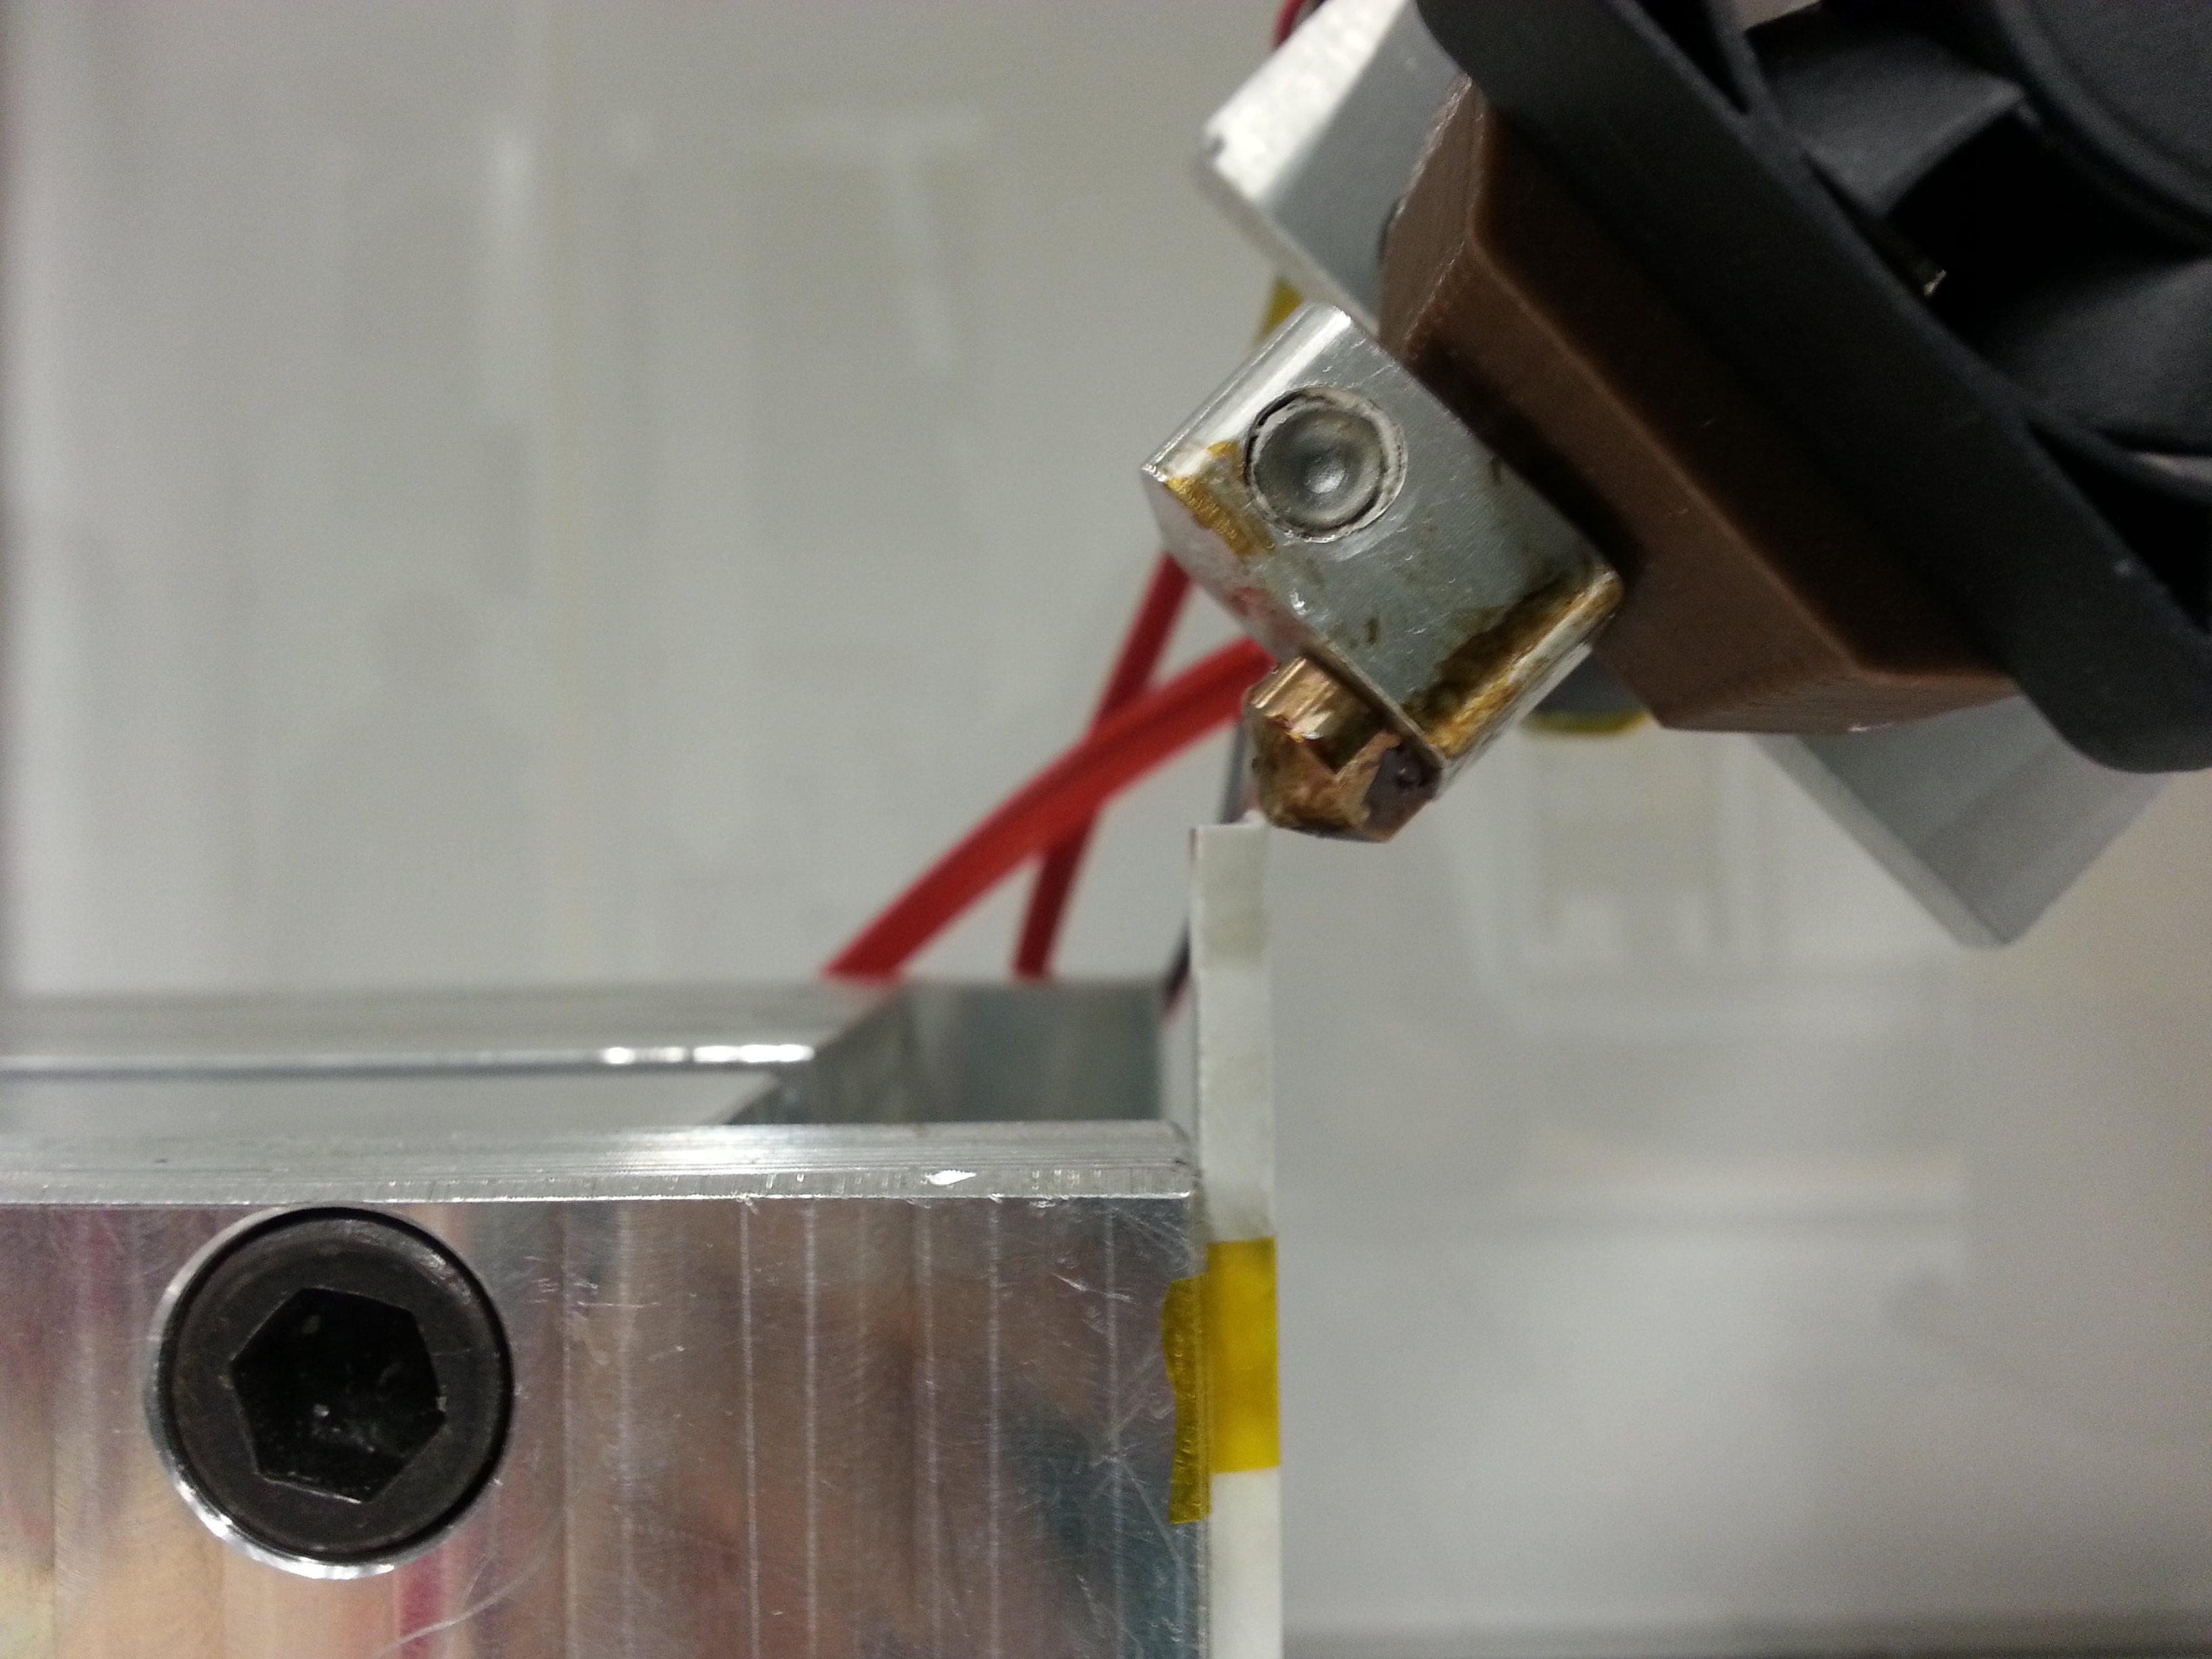
\includegraphics[width=.8\linewidth]{figures/tool-pt-1-close}
    \end{subfigure}
    \caption{Tool Frame reference position 1}
    \label{fig:tool-pt-1}
\end{figure}

\begin{figure}
    \centering
    \begin{subfigure}{.5\textwidth}
        \centering
            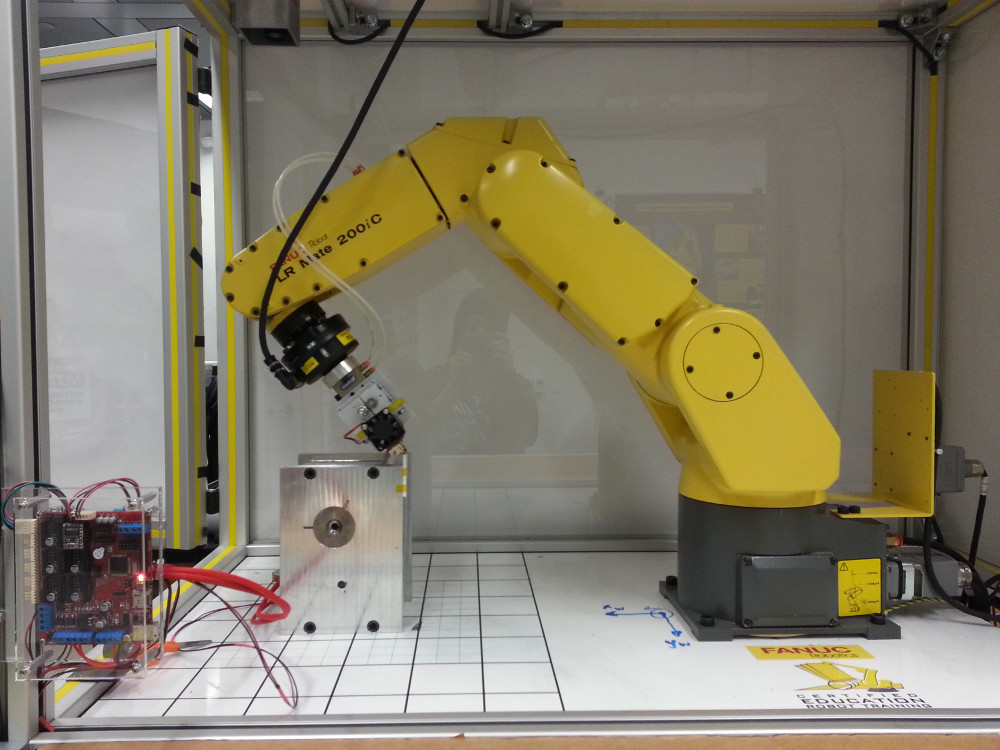
\includegraphics[width=.8\linewidth]{figures/tool-pt-2}
    \end{subfigure}%
    \begin{subfigure}{.5\textwidth}
        \centering
        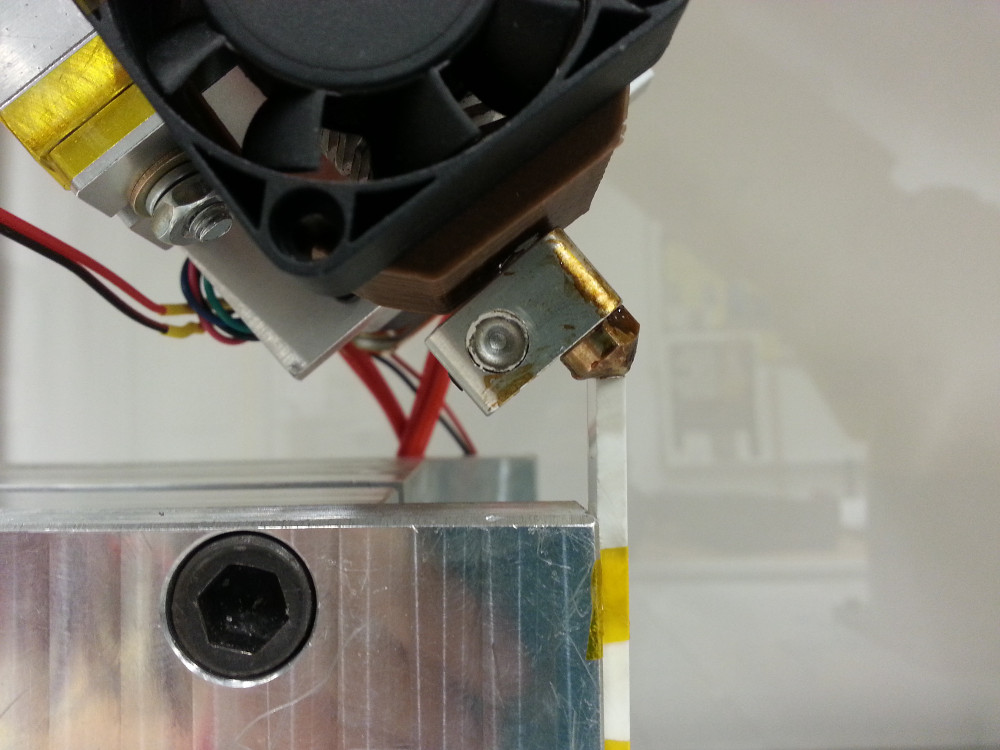
\includegraphics[width=.8\linewidth]{figures/tool-pt-2-close}
    \end{subfigure}
    \caption{Tool Frame reference position 2}
    \label{fig:tool-pt-2}
\end{figure}

\begin{figure}
    \centering
    \begin{subfigure}{.5\textwidth}
        \centering
        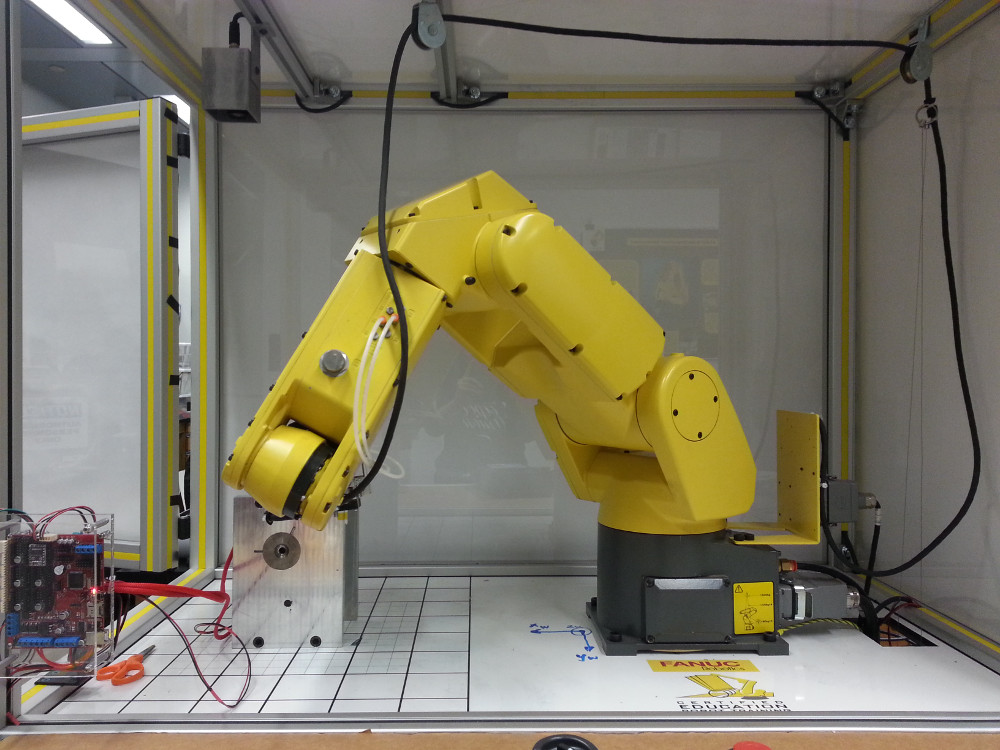
\includegraphics[width=.8\linewidth]{figures/tool-pt-3}
    \end{subfigure}%
    \begin{subfigure}{.5\textwidth}
        \centering
        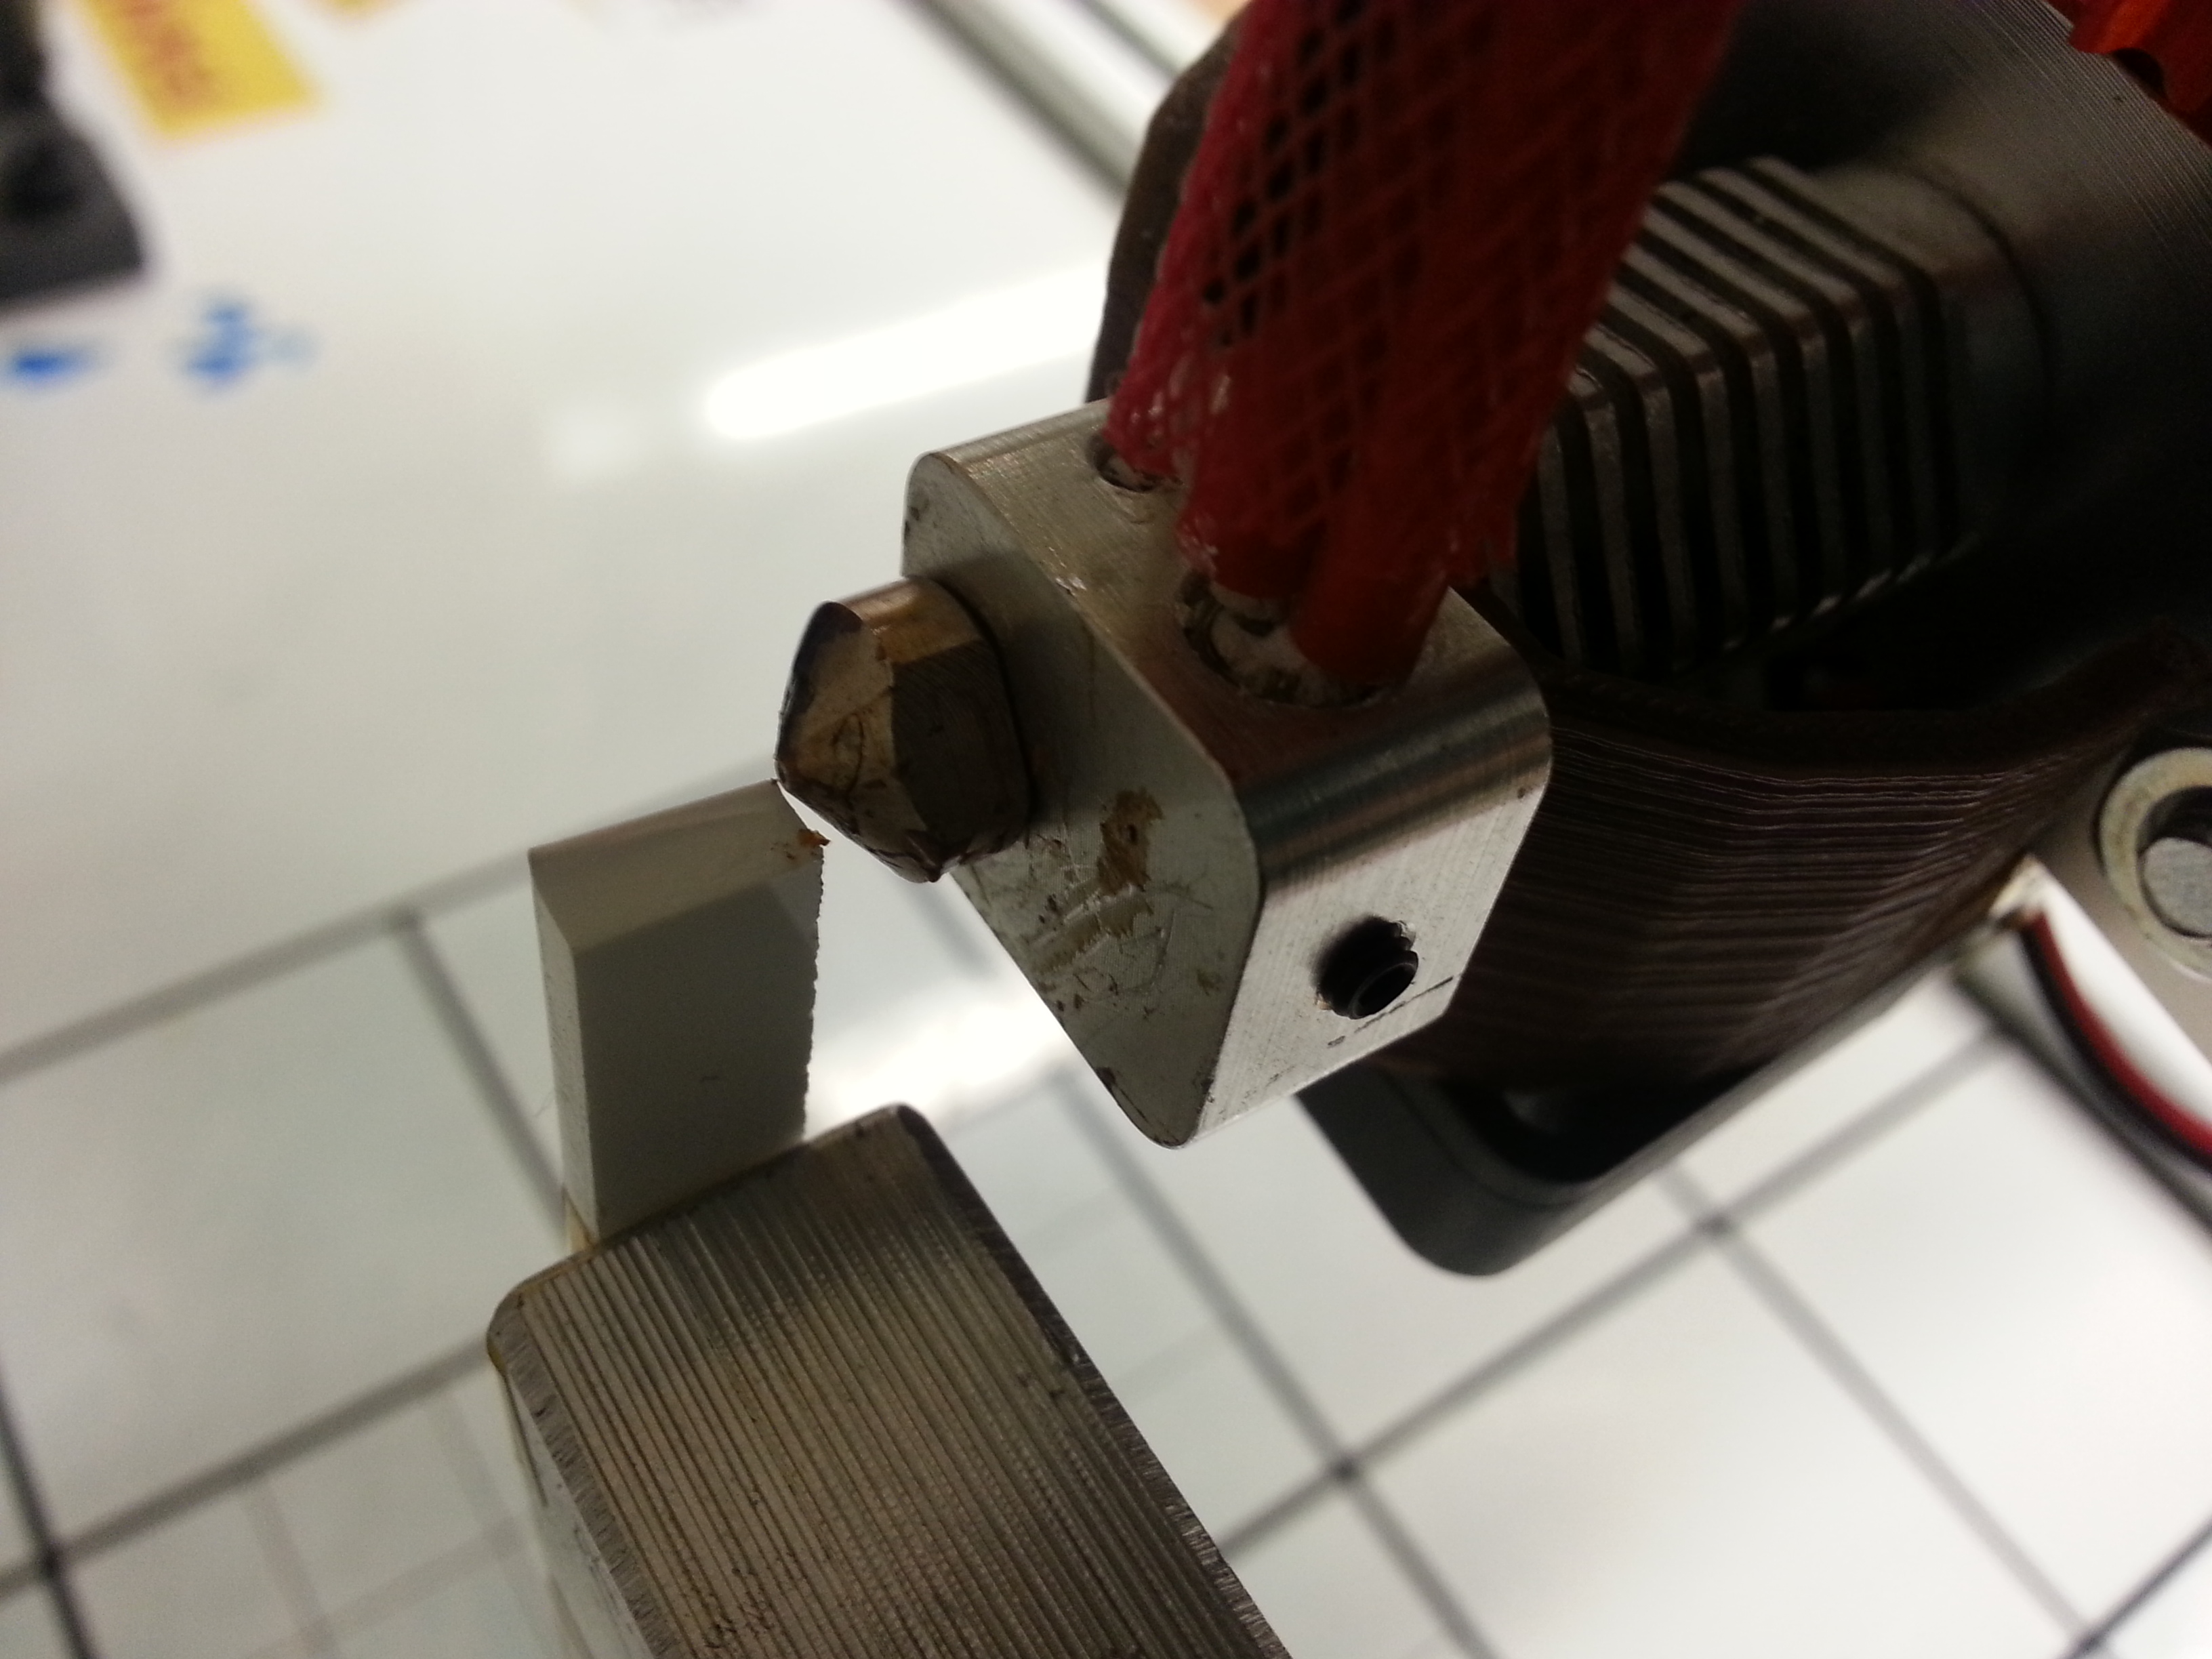
\includegraphics[width=.8\linewidth]{figures/tool-pt-3-close}
    \end{subfigure}
    \caption{Tool Frame reference position 3}
    \label{fig:tool-pt-3}
\end{figure}

Figure~\ref{fig:utool} shows the teach pendant screen after using the Three Point Method. The left display lists defined tool frames; the right display lists the position and angle coordinates of the printer hot end tool frame. These coordinates are defined with respect to the end-of-arm frame, because the tool is expected to be attached to the end of the robot arm. The \verb|USED| flags indicate that all three points have been defined. 

\begin{figure}
    \centering
    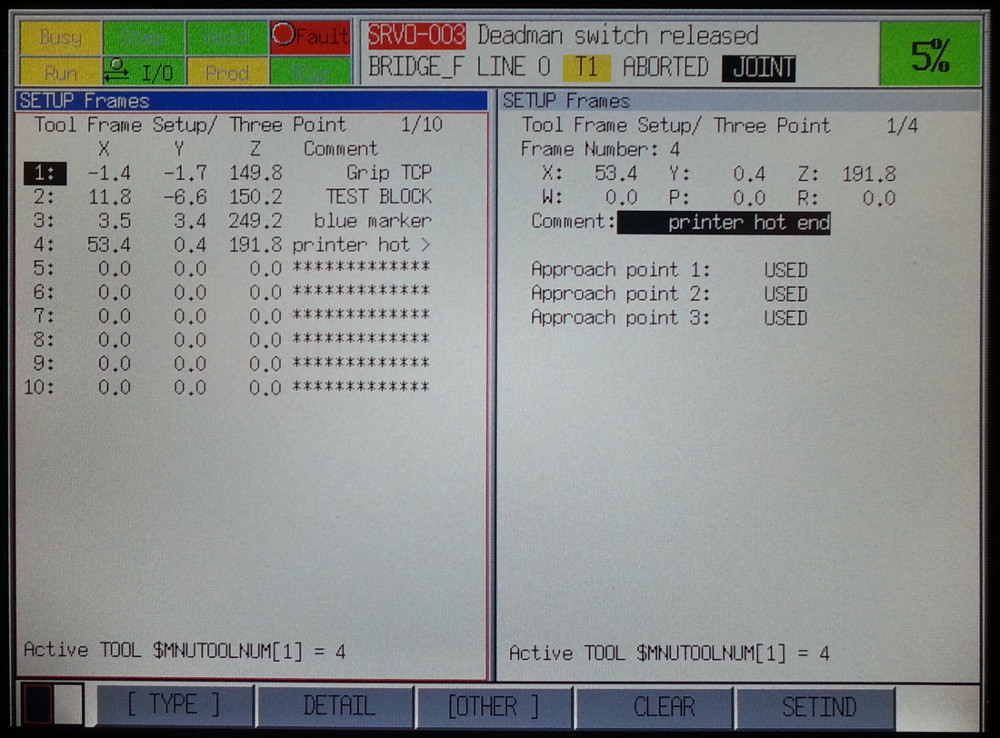
\includegraphics[width=.8\linewidth]{figures/tp-screens/utool}
    \caption{Teach pendant user tool frame setup screen.}
    \label{fig:utool}
\end{figure}

\subsubsection{User frame}
The new user frame is attached to the robot workspace and is used as the coordinate system for 3D printing. The user frame was defined using the Direct List Method described in \cite[sec~3.9.2]{lr-handling-tool}. Assuming the dry-erase board surface would be used for printing, and that it lies in the x-y plane of the robot World frame\footnote{Both assumptions may become problematic if the board surface is not sufficiently flat or parallel to the x-y plane of the World frame. A new print surface and User frame may be required. Existing FDM (closed- and open-source) solutions may give clues.}, the z-coordinate of the new user frame was determined by touching the nozzle tip to the board and recording the z-coordinate of the robot in the World frame. A sheet of paper was placed under the nozzle tip to indicate a touch, shown in Figure~\ref{fig:nozzle-touch}. 

\begin{figure}
    \centering
    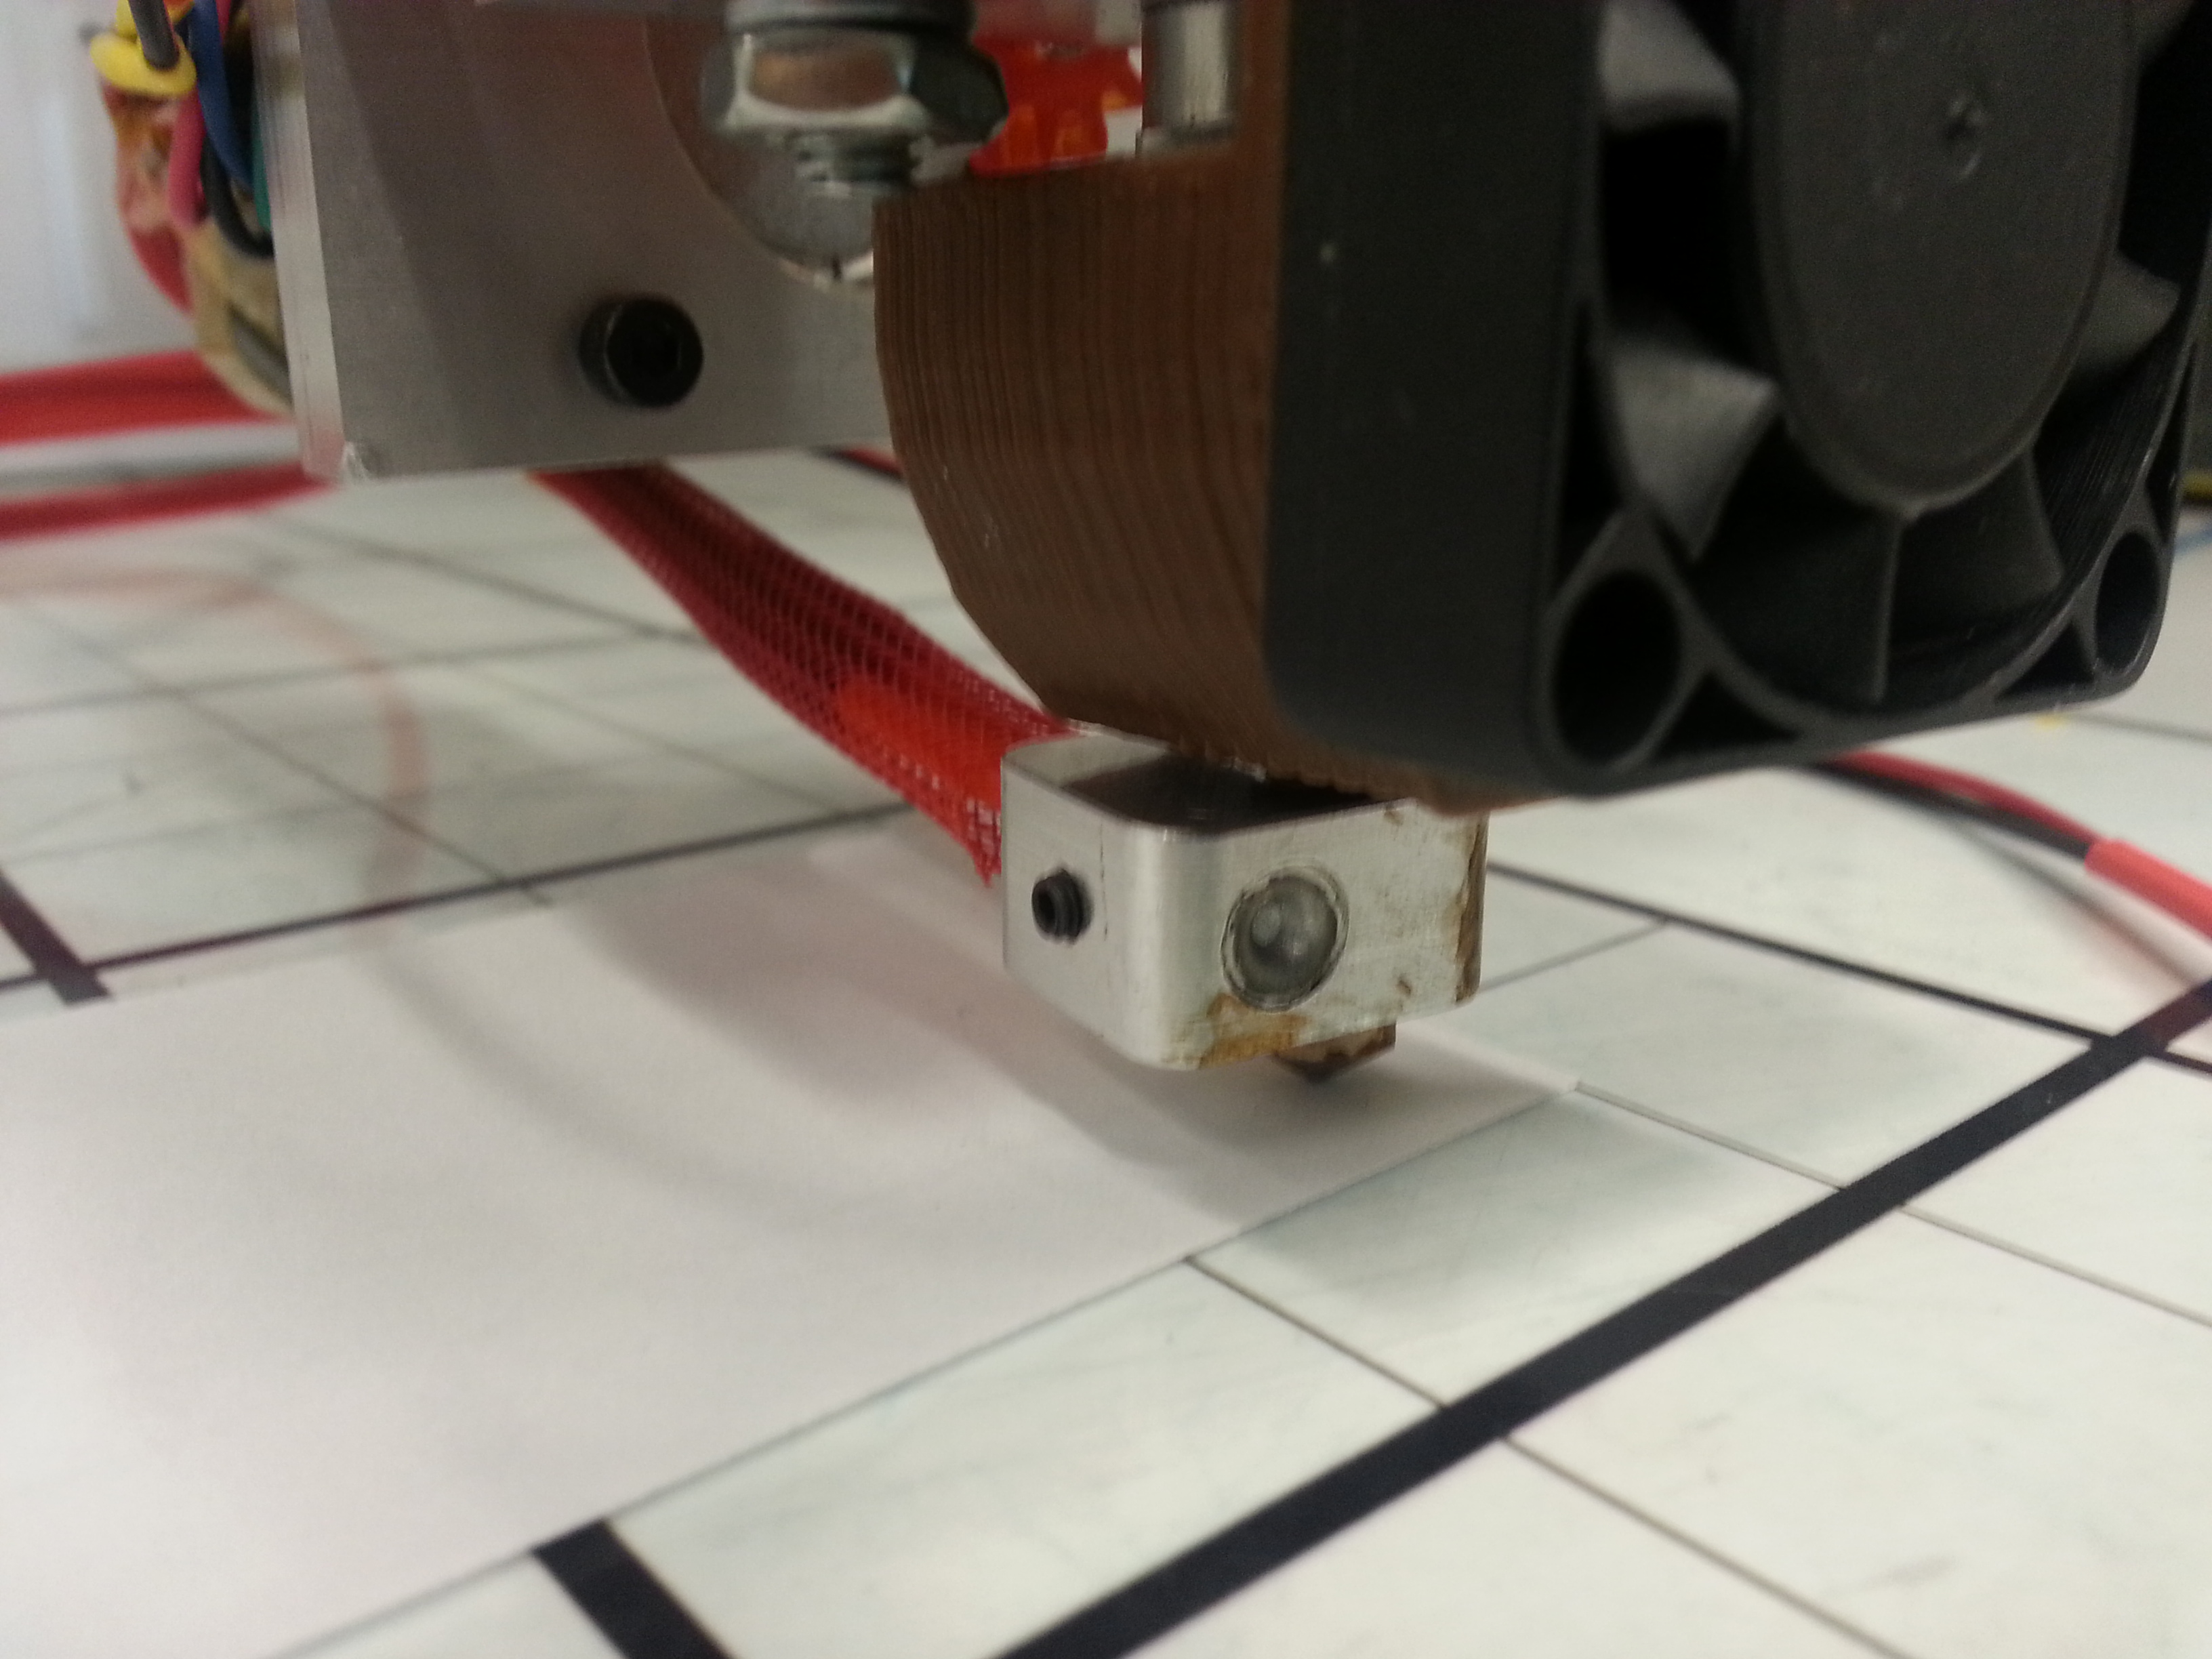
\includegraphics[width=.8\linewidth]{figures/nozzle-paper}
    \caption{User frame nozzle touch test}
    \label{fig:nozzle-touch}
\end{figure}

Figure~\ref{fig:uframe} show the teach pendant screen after using the Direct Entry Method to define User Frame 4. The left display lists defined User Frames; the right display lists the entered position and angle coordinates of the printing space User Frame. These coordinates are defined with respect to the World frame, which is fixed to the base of the robot arm. Note that here \(R=-90\si{\degree}\) in order to relieve some stress on the extruder wires.

\begin{figure}
    \centering
    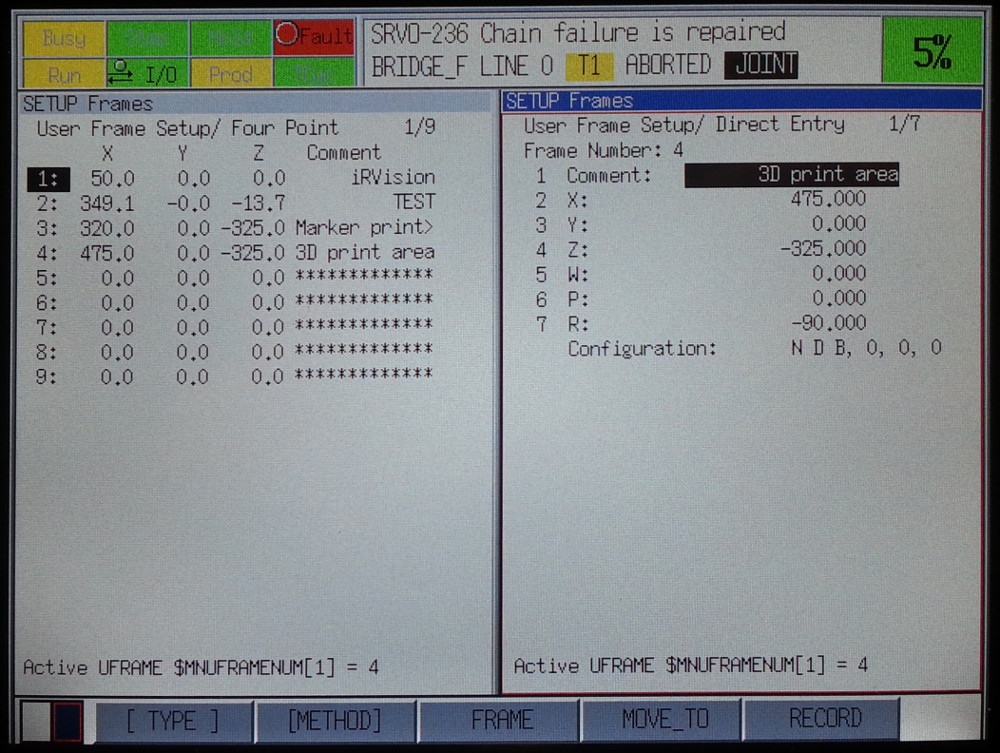
\includegraphics[width=.8\linewidth]{figures/tp-screens/uframe}
    \caption{Teach pendant user tool frame setup screen.}
    \label{fig:uframe}
\end{figure}

\subsection{Programming}
Unlike most other modern computer programming, programming the FANUC robot is done through the teach pendant unless the user has access to certain additional FANUC software packages that provide Windows compilers for TP and its cousin language KAREL. The programs are written in the TP (Teach Pendant, of course) language provided by FANUC, which provides basic motion instructions and low-level mathematical and control flow instructions. Given the slow nature of programming, testing, and debugging through the teach pendant interface, there is a special incentive to write as few lines of instructions as possible. 

A program called \verb|bridge_f.tp| was written to generate the extruder motion for printing the curved-layer test specimen described in Figure~\ref{fig:fea-body-geometry}. Normally, FANUC robot programs are created largely by teaching points, which entails manually jogging the robot to each desired path point and recording them individually. This method ensures that each teach point is exactly where and in what arm orientation the user intends. However, this method is not sustainable for 3D printing parts, which may have hundreds or thousands of individual path points to successfully reach. Fortunately, the outer geometry and one possible fiber orientation for the desired curved-layer specimen lead to a toolpath design that, by symmetry, requires very few path points need to be defined and verified. 

The text of the \verb|bridge_f.tp| program is shown below\footnote{Unfortunately, there does not seem to be a way to export plaintext TP code from the teach pendant. This program text was manually transcribed from the teach pendant screen. Pseudo-comments were added later.}, along with Figure~\ref{fig:bridge-edit}, which shows the teach pendant screen during program editing. Explanations of the toolpath geometry and motion instructions follow.

\begin{verbatim}
 1:  UFRAME_NUM=4                            // set user frame
 2:  UTOOL_NUM=4                             // set user tool frame
 3:  R[4:layer num]=0                        // reset layer counter
 4:  PR[12:layer frame RW]=                  // set layer RW (read+write) frame 
  :  PR[11:layer frame R]                       position register   
 5:  R[5:contour num]=0                      // reset contour counter
 6:  PR[13,2:contour offset]=0               // reset contour offset
 7:  R[7:contour incr dir]=(-1)              // reset contour increment direction
 8:  TOOL_OFFSET_CONDITION                   // set tool offset condition to  
  :  PR[13:contour offset]                      contour offset
 9:  LBL[2]                                  // label 2: layer loop
10:  UFRAME[4]=PR[12:layer frame RW]         // set user frame to incremented 
  :                                             layer frame
11:  LBL[1]                                  // label 1: contour loop
12:J  P[1] 100% FINE Tool_Offset             // joint move to point 1
13:J  P[2] 100% FINE Tool_Offset
14:C  P[3] Tool_Offset                       // circular interpolation 
  :   P[4] 250mm/sec FINE Tool_Offset           thru pt 3 to pt 4
15:C  P[5] Tool_Offset
  :   P[6] 250mm/sec FINE Tool_Offset
16:C  P[7] Tool_Offset
  :   P[8] 250mm/sec FINE Tool_Offset
17:J  P[9] 100% FINE Tool_Offset
18:  PR[13,2:contour offset]=(               // increment contour offset 
  :  PR[13,2:contour offset]+                   position register
  :  R[6:contour incremnt]*
  :  R[7:contour incr dir]))
19:J  P[9] 100% FINE Tool_Offset
20:C  P[8] Tool_Offset
  :   P[7] 250mm/sec FINE Tool_Offset
21:C  P[6] Tool_Offset
  :   P[5] 250mm/sec FINE Tool_Offset
22:C  P[4] Tool_Offset
  :   P[3] 250mm/sec FINE Tool_Offset
23:J  P[2] 100% FINE Tool_Offset
24:J  P[1] 100% FINE Tool_Offset
25:  R[5:contour num]=R[5:contour num]+1     // increment contour counter
26:  IF R[5:contour num]>=31,JMP LBL[3]      // don't increment after last 
                                                contour pair
27:  PR[13,2:contour offset]=(
  :  PR[13,2:contour offset]+
  :  R[6:contour incremnt]*
  :  R[7:contour incr dir]))
28:  JMP LBL[1]
29:  LBL[3]
30:  R[4:layer num]=R[4:layer num]+1         // increment layer counter
31:  PR[12,3:layer frame RW]=                // increment layer frame 
  :  PR[12,3:layer frame RW]+.1                 position register
32:  R[7:contour incr dir]=                  // invert contour increment
  :  R[7:contour incr dir]*(-1)                 direction
33:  IF R[4:layer num]<31,JMP LBL[2]
[END]
\end{verbatim}


\begin{figure}
    \centering
    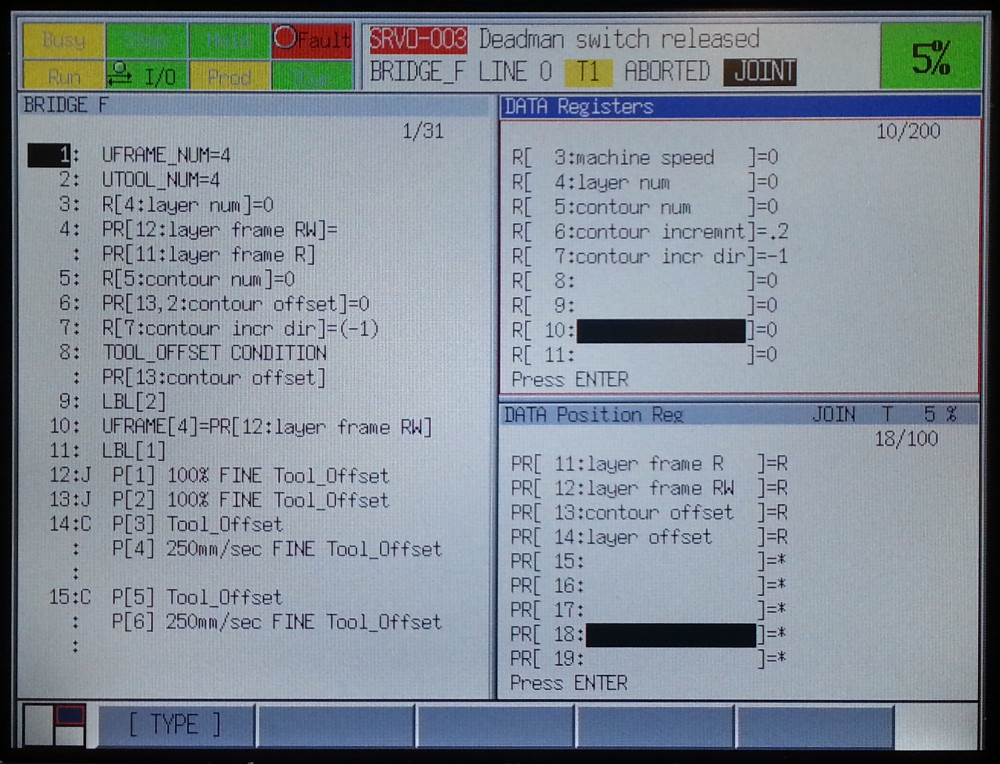
\includegraphics[width=.8\linewidth]{figures/tp-screens/bridge-edit}
    \caption{Teach pendant TP program editing screen.}
    \label{fig:bridge-edit}
\end{figure}

\subsubsection{Motion commands}
In this program, only joint (denoted by J) and circular interpolation (denoted by C) motions are used. The joint motions specify the start and end point of a move, but do not control the tool path or attitude between the start and end point \cite[sec~4.3.1]{lr-handling-tool}. Thus,if a linear attitude-controlled move is required, the linear (L) move is normally used. However, the nominally straight-line moves in this program are relatively short, about 16mm, so it is predicted that any nonlinearities introduced by the joint motion will be trivial. The joint motions may be replaced by linear motions if they present a problem in print testing. The circular motions specify a start point, an intermediate point, and an end point, all with associated tool attitudes. During circular motions, the tool path and attitude are defined. That aspect of the circular instruction will be important for two reasons: first, the tool attitude may be kept normal to the print surface during curved-layer moves, avoiding possible nozzle interference problems; second, the tool attitude control will allow adjacent curved-layer toolpath points to be generated easily, as explained in Section~\ref{sec:point-gen}.

\subsubsection{Data registers}
Data registers are portions of memory used like variables for storing numerical data\cite[sec~7.3]{lr-handling-tool}. In \verb|bridge_f.tp|, they are used as counters, distance values, and flagsvia register instructions\cite[sec~4.5.1]{lr-handling-tool}. The data registers used in the program are listed on the \verb|DATA Registers| screen in the top-right display in Figure~\ref{fig:bridge-edit}. 

\subsubsection{Position registers}
Position registers are like data registers; they are used to hold position data\cite[sec~7.4]{lr-handling-tool}. Each position register holds six coordinates \((X,Y,Z,W,P,R)\), \((X,Y,Z)\) being the position coordinates and \((W,P,R)\) being the orientation or attitide coordinates,  In \verb|bridge_f.tp|, they are used not only for defining toolpath points, but also for adjusting the User Frame and defining the Tool Offset, the use of which is described in Section~\ref{sec:pos-incr}. 

\subsubsection{Position increments}
\label{sec:pos-incr}
\subsubsection{Control flow}
\subsubsection{Toolpath point generation}
\label{sec:point-gen}

\subsection{Speed output signal}
\begin{verbatim}
1:	R[3:machine speed]=$SCR_GRP[1].$MCH_SPD
2:	AO[1]=R[3:machine speed]
[END]
\end{verbatim}

